\documentclass[12pt]{article}

\usepackage[fleqn]{amsmath}
\usepackage{amssymb}
\usepackage{amsthm}
\usepackage{graphicx}
\usepackage{float}
\theoremstyle{plain}     %------- 'regular' theorem types
\newtheorem{thm}{Theorem}[section]
\newtheorem{cor}[thm]{Corollary}
\newtheorem{lemma}[thm]{Lemma}
\newtheorem{prop}[thm]{Proposition}
\newtheorem{example}[thm]{Example}
\newtheorem{exer}[thm]{Exercise}
\newtheorem{define}[thm]{Definition}
\usepackage[top=2cm, left=2cm, right=2cm]{geometry} 
\usepackage{parskip}
\setlength{\parindent}{0in}
\usepackage{floatflt}
\usepackage{multicol}
\usepackage{tabu}
\usepackage[hidelinks]{hyperref}
\hypersetup{
	urlcolor=blue}

%%%%%%%%%%%%%%%%%%%%%%
%%%%%%%%%%%%%%%%%%%%%%%
%%%%%%%%%%%%%%%%%%%%%%%%
\begin{document}
\large
%subject
City Semester%  \hspace{8cm} Name:\makebox[6cm]{\hrulefill}
\\
%specific topic
Problem Set \#3\\
\normalsize 
%\emph{Complete all work on a separate sheet of paper with exercises clearly labeled and all reasoning and work given.}\\[.5cm]
\emph{Show all work for full credit.}\\
\begin{enumerate}
	\item Calculate the following summary statistics for the given data set: $\{1,2,2,3,3,5,9,11\}$
		\begin{enumerate}
			\item Find $\overline{X}$.
			\item Find the variance $\sigma^2$.
			\item Find the standard deviation $\sigma$.
			\item Explain how why $\sigma$ is used as a measure of spread.
			\item Give the five number summary for this data set.
			
		\end{enumerate}
	
	\item 2.	A few years ago then mayor Bloomberg made it a personal quest to control what New Yorkers eat in an effort to improve health – largely motivated by statistics like this: the percentage of New York State adults who are overweight or obese increased from 42\% in 1997 to 60\% in 2008. 
(source: NYS Dept of Health)

New Yorkers compare slightly more favorably to US citizens as a whole, but not much. The graph below shows the percent of the population in various countries that are overweight.  
	\begin{figure}[H]
		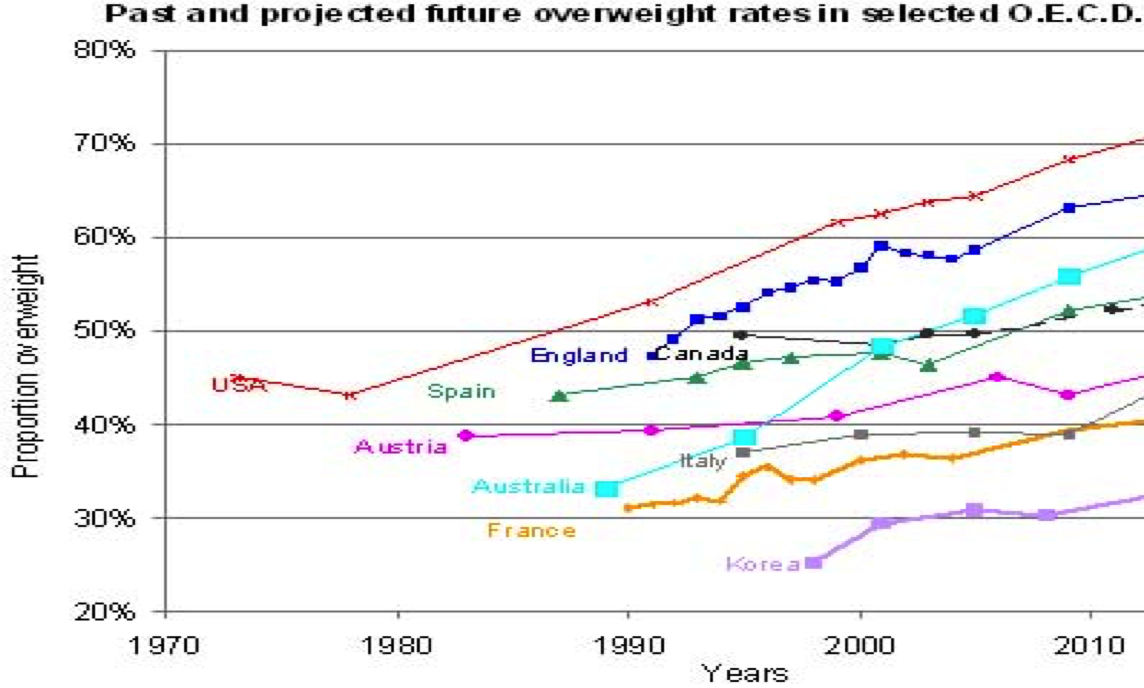
\includegraphics[scale=.75]{1.png}
	\end{figure}
		\begin{enumerate}
			\item According to the graph, what was the approximate percentage of the US population that was overweight in 1995?  Is your answer an interpolation or an extrapolation?
			\item The graph is cut off at about 2013.  Based on the portion of the graph that is shown, about what percent of the US population do you think will be overweight in 2020?  Is your answer an interpolation or an extrapolation?
			\item If you are confident this relationship is linear what portion of the US population do you think will be overweight in 2100?  How did you arrive at that answer? Are you more or less confident in this answer than in part b?

		\end{enumerate}
		
	\item 
\includegraphics[scale=.1]{fathom.png} Average Hourly Wage for workers in NYC 2009 to 2013 
		\begin{enumerate}
			\item Open the Fathom data file “AvgHourlyEarnings-NYC” and fit a linear model to the data with “Months since Jan09” as the input and “AverageHourlyEarning” as the output.
			\item Right-click on the graph after you’ve plotted your function and choose “Make Residual Plot” (near the bottom).  What is the residual plot showing you?  
			\item Looking at the residual plot, do you think a linear model is appropriate for this data?  Do you think your model is a useful predictor of data values?  Explain.

		\end{enumerate}
	
	\item 
\includegraphics[scale=.1]{fathom.png} Revisit “Average Hourly Wage” in NYC 2009 to 2013 
		\begin{enumerate}
			\item Open data file “AvgHourlyEarnings-NYC” and fully “analyze the data” according to the 5 steps shown on the slides (you can use your model from the last problem set if you still have it).
			\item Write a sentence that explains the meaning of the slope of your linear model within the context.
			\item Use the model to predict what the Average Hourly Wage would be for Jan 2015 (72 months after Jan ’09) 
			\item According to the slope of the model, what was the average yearly change in hourly wage?
		\end{enumerate}
	
	\item 
\includegraphics[scale=.1]{fathom.png} Lastly, let's look at obesity rates in NY state. Keep in mind this is obesity as measured by BMI. There are many problems with this measure.
		\begin{enumerate}
			\item Open data file NY obesity and generate a scatterplot with years on the $x$-axis and percentage of people with BMI $>$ 30 on the $y$-axis.
			\item Write a sentence explaining the meaning of the slope of your linear regression line in the context of the data.
			\item Use the model to predict obesity rates is 2020. Compare with your results in problem 2.
			\item Look at the residual plot of your least squares regression line. Are you confident that the data is linear? Explain.
		\end{enumerate}
	
	
\end{enumerate}
	
\end{document} 